\documentclass[12pt]{article}

\usepackage[english]{babel}
\usepackage[utf8x]{inputenc}
\usepackage{amsmath}
\usepackage{graphicx}
\usepackage{authblk}
\usepackage{natbib}
\bibpunct{(}{)}{;}{author-year}{}{,}

\title{Host diversity increases symbiont diversity and reduces transmission}

\author[1]{Maxwell B. Joseph} 
\author[2]{Joseph R. Mihaljevic}
\author[1]{Pieter T. J. Johnson}
\affil[1]{Ecology and Evolutionary Biology, University of Colorado, Boulder}
\affil[2]{Ecology and Evolution, University of Chicago}
\date{}
\renewcommand\Affilfont{\itshape\small}

\begin{document}
\maketitle

\begin{abstract}
Your abstract.
\end{abstract}

\section{Introduction}

Debate around effect of host diversity on disease. 
Increased availability of microbial data. 
Need for theoretical framework to make sense of data and predict future observations.

General strategy: 
- formalize the notion that host infection dynamics potentially have similarities to free living metacommunity dynamics
- develop a model that can capture the complexity of multi-host, multi-symbiont systems
- advantages (better realism, adequate complexty)
- disadvantages (less tractable than a simple analytical mathematical model)

\section{Methods}

We developed a stochastic continuous-time agent-based model for the dynamics of host-symbiont communities in local habitat patches that are made up of a finite number of cells that may be occupied by hosts. 
The local habitat patches are all considered to be equivalent with respect to host colonization, reproduction, and death. 
Multiple host species exist within a regional pool, and each patch experiences a constant rate of host colonization, which is equal for all host species, although there is no displacement of occupying hosts by colonizing hosts. 
Once a host colonizes a patch, it then has some rate of reproduction and of death that is constant among host species.

Multiple types of symbionts occur in the regional pool and attempt to colonize host individuals with a constant rate. 
Host species vary in traits relevant to symbiont establishment probability. 
We assume for simplicity that this variation is unidimensional, as would be the case if there were one primary niche axis for the symbionts (e.g. pH of the host gut). 
Symbiont niches are represented as univariate Gaussian functions with niche optima and breadths (means and variances, respectively), such that the probability of successful establishment on an individual host is a function of the host's value along the niche axis (Figure 1). 
Each symbiont has the same total probability of colonizing in the regional pool as a result of adjusting the niche functions of symbiont species with niche optima near the boundaries of  the niche space of the regional pool (e.g. symbiont 2 in Figure 1).

Every individual host has some constant probability of a symbiont from the regional pool attempting to infect, with an infection success probability being drawn from the symbiont niche function, given the host species condition. 
If a symbiont successfully colonizes a host, it becomes part of the local community and can either be extirpated through host recovery or persist by transmitting to other hosts (Figure 2). 
Every infected host has some recovery rate that is assumed constant across all species. 
Transmission occurs according to either density-dependent or frequency-dependent dynamics, where contact rates between infected and susceptible hosts are represented by $\beta S I$ or $\dfrac{\beta S I}{N}$, respectively, where $S$ is the number of susceptible hosts, $I$ is the number of infected hosts, $N$ is the total number of hosts, and $\beta$ is the per capita contact rate. 
For the case with static host communities, $N$ is constant, so that the dynamics of density and frequency dependent transmission are not appreciably different, other than a potential reduction in contact rates with frequency-dependent transmission (though this decrease can be offset by increasing $\beta$, leading to identical contact rates). 
Note that these terms are representing contacts between hosts that could result in transmission, but that the success of transmission still depends on the relationship between the condition of the susceptible host relative to the symbiont niche. 
Hosts are infected by symbionts at a particular location that can only be occupied by one type of symbiont (no co-infection). 

We implement the previous model via stochastic simulation, generating continuous-time Markov chains in high-dimensional space, where the dimensions represent the states (number of hosts of each species, and the symbionts that infect each individual). 
Although continuous-time Markov processes are more difficult computationally than discrete-time formulations, they have the advantage of not requiring an arbitrarily specified order of events at each time step. 
Instead, the order of events emerges from the rates of each potential process via the Gillespie algorithm \citep{Gillespie1976}. 
Specifically, given the state of the system at any time point, every potential event that could happen is represented by some rate $r_e$ for events $e = 1, ..., E$. 
The total rate of events is simply the sum of the component rates $r_{tot} = \sum_{1}^{E} e_r$, and the time until an even happens is exponentially distributed, with overall rate parameter $r_{tot}$. 
This provides a way to generate the timepoints stochastically, and given some time of an event happening, the specific event is be selected with probability $\dfrac{e_r}{r_{tot}}$. 
This algorithm results in an exact solution for the stochastic process of interest. 

Next, we consider a local habitat patch that contains populations of hosts that are infected by symbionts. 
The host populations are open, with deaths, births, emigration and immigration.
Symbionts can still be transmitted among host individuals, or colonize from outside of the local host population from the regional pool, and each infected host as a recovery rate as before. 
There are multiple host species in a regional pool that can colonize the local community, and they vary in traits that are relevant to symbiont infection, but the communities are otherwise neutral, in that all host species have equal colonization, reproduction, and death rates. 
Hosts occur in a homogenous landscape, and can colonize the local habitat from the regional pool, reproduce, and die. 
Offspring attempt to disperse to a random habitat patch, and if it is unnoccupied, they successfully colonize.

Symbionts can be parasitic, commensal, or mutualistic through their effects on host survival.
To ensure that we can investigate a range of conditions, we modify the host survival rate $r$ as a function of infection:

$$r = d(1 + \beta_d * I(infected))$$

where $d$ is the background death rate, and $I(infected)$ is an indicator function that returns $1$ if an individual host is infected. 
The parameter $\beta_d$ controls the effect of infection on survival. 
When $\beta_d = 0$, the symbiont has no effect on survival, positive values impose increases in the death rate, and values in the interval $(-1, 0]$ represent decreases in death rate. 
We would expect that by being virulent and killing hosts, persistence in a local host community becomes more difficult because symbionts are destroying their resource, wheras mutualists can persist more easily because by increasing the longevity of their hosts, infected hosts can produce more offspring over the course of their lifetime.
As a consequence, for a given level of host diversity, parasites may have a lower value of expected value of richness than commensals, which have a lower expected richness compared to mutualists. 

\section{Results}

Host diversity increased symbiont diversity, but the effect was non-linear (Figure 4). 
Furthermore, although we did observe a similar 2nd degree polynomial type of relationship, we did not observe a unimodal relationship between host and symbiont diversity across any range of parameter values. 

As expected, when symbionts reduced host longevity, persistence within the host community becomes less probable for each symbiont species, resulting in a reduction in mean symbiont richness. 
Symbionts that increased host longevity showed the reverse pattern: persistence becomes more likely when symbionts are mutualists, resulting in higher mean symbiont richness (Figure 5). 

\section{Discussion}

Static host communities 
- extension of free living species concept, but not so applicable
- observed unimodal relationship

Dynamic host communities
- more realistic
- difference between potential vs. realized host richness
- not as strong unimodal relationships observed, because it's very unlikely to have tons of very small, very different host populations (small populations face a higher risk of stochastic extinctions)

See Dunn et al. 2010 for non-linear relationship

See Rotstock et al. 2014 for similar resolution of paradox

\bibliographystyle{plainnat}
\bibliography{Mendeley}

\newpage

\section*{Figure 1}

\begin{figure}[ht]\centering
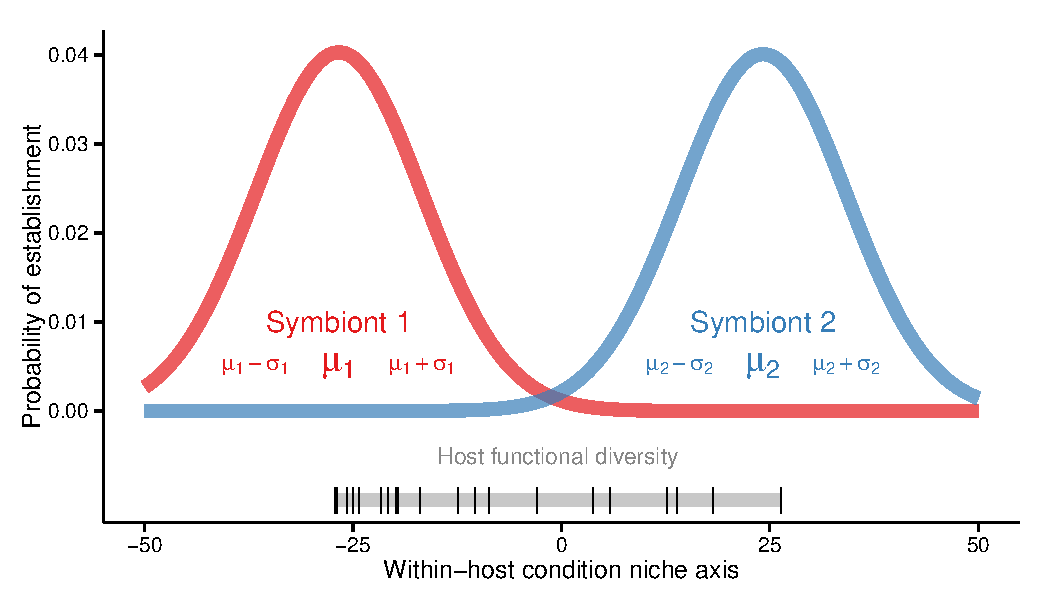
\includegraphics[width=\linewidth]{fig/niche.pdf}
\caption{Commensal symbionts, all same niche width}
\label{fig:fig/fig1}
\end{figure}

\newpage

\section*{Figure 1}

\begin{figure}[ht]\centering
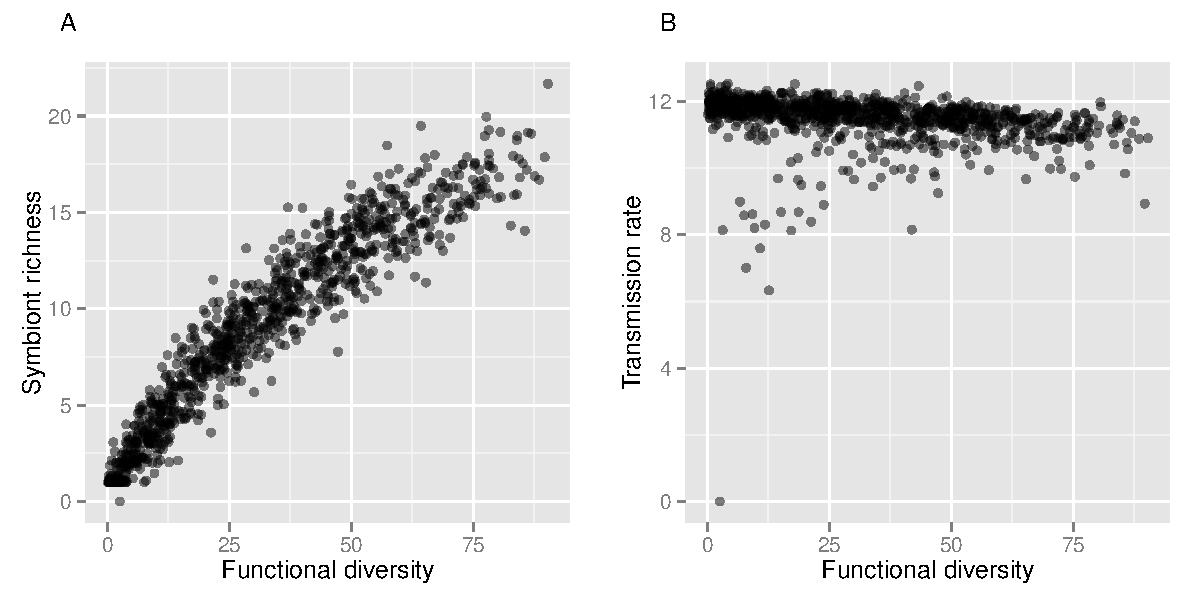
\includegraphics[width=\linewidth]{fig/fig1.pdf}
\caption{Commensal symbionts, all same niche width}
\label{fig:fig/fig1}
\end{figure}

\newpage

\section*{Figure 2}

\begin{figure}[ht]\centering
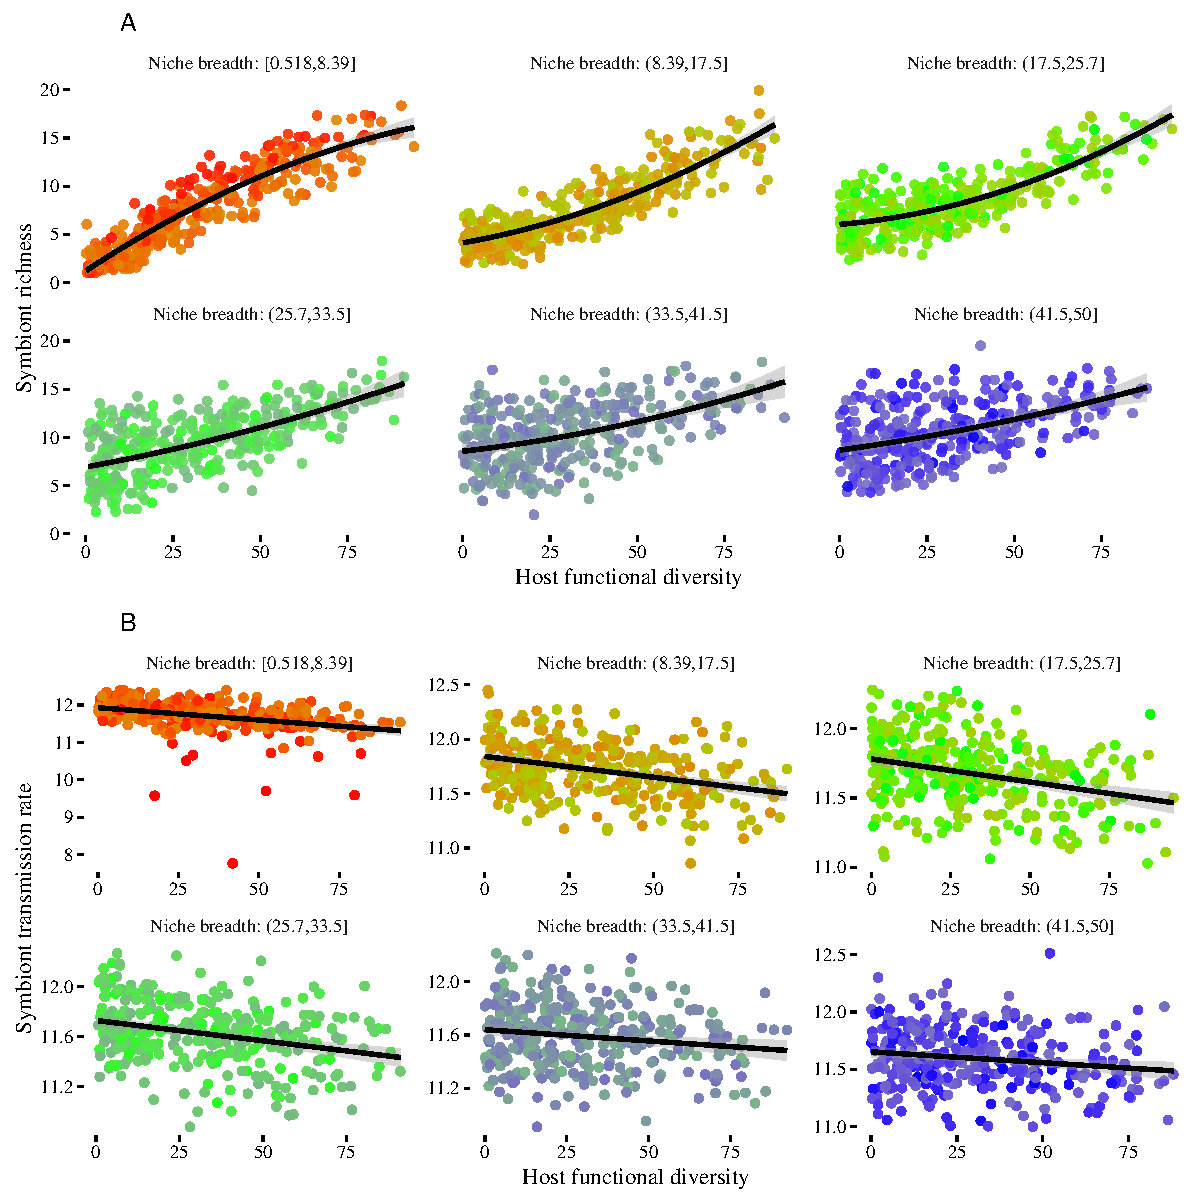
\includegraphics[width=\linewidth]{fig/fig2.pdf}
\caption{Varying niche width, but constant within symbiont community}
\label{fig:fig2}
\end{figure}

\newpage

\section*{Figure 3}

\begin{figure}[ht]\centering
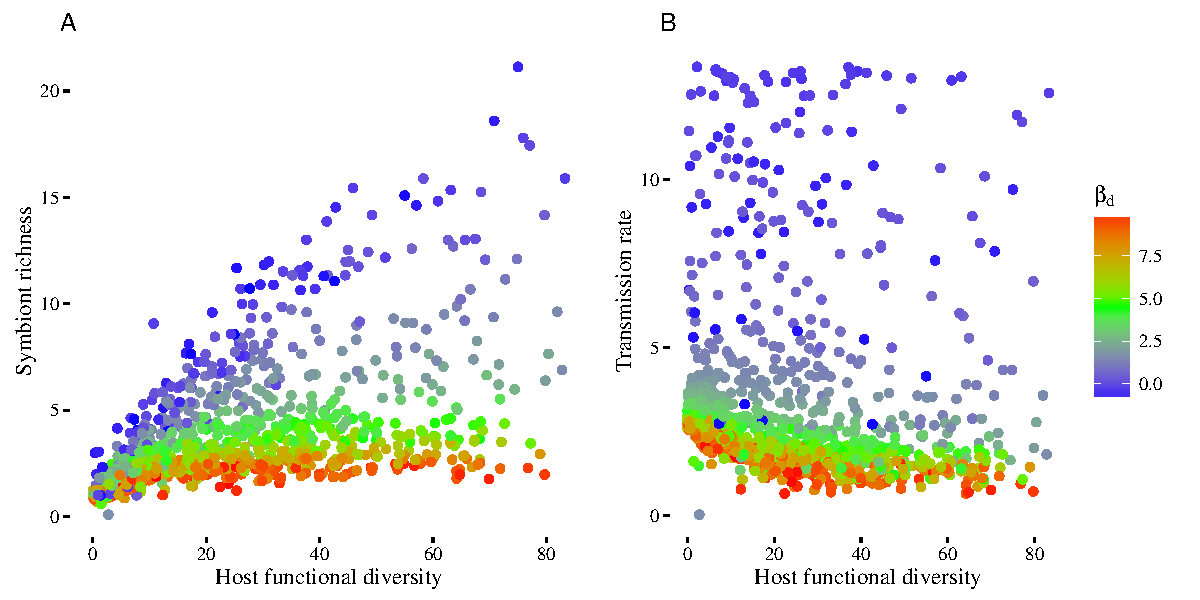
\includegraphics[width=\linewidth]{fig/fig3.pdf}
\caption{Varying fitness consequences, but constant within symbiont community}
\label{fig:fig3}
\end{figure}

\newpage

\section*{Figure 4}

\begin{figure}[ht]\centering
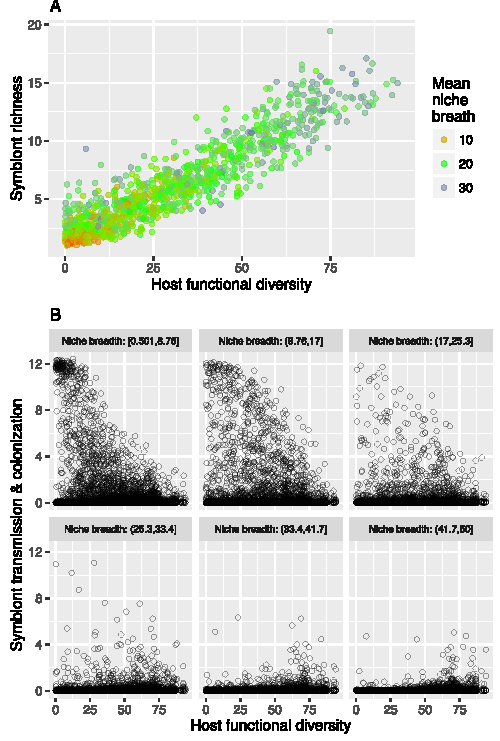
\includegraphics[width=\linewidth]{fig/fig4.pdf}
\caption{Mixed niche breadths within symbiont community}
\label{fig:fig4}
\end{figure}

\newpage

\section*{Figure 5}

\begin{figure}[ht]\centering,
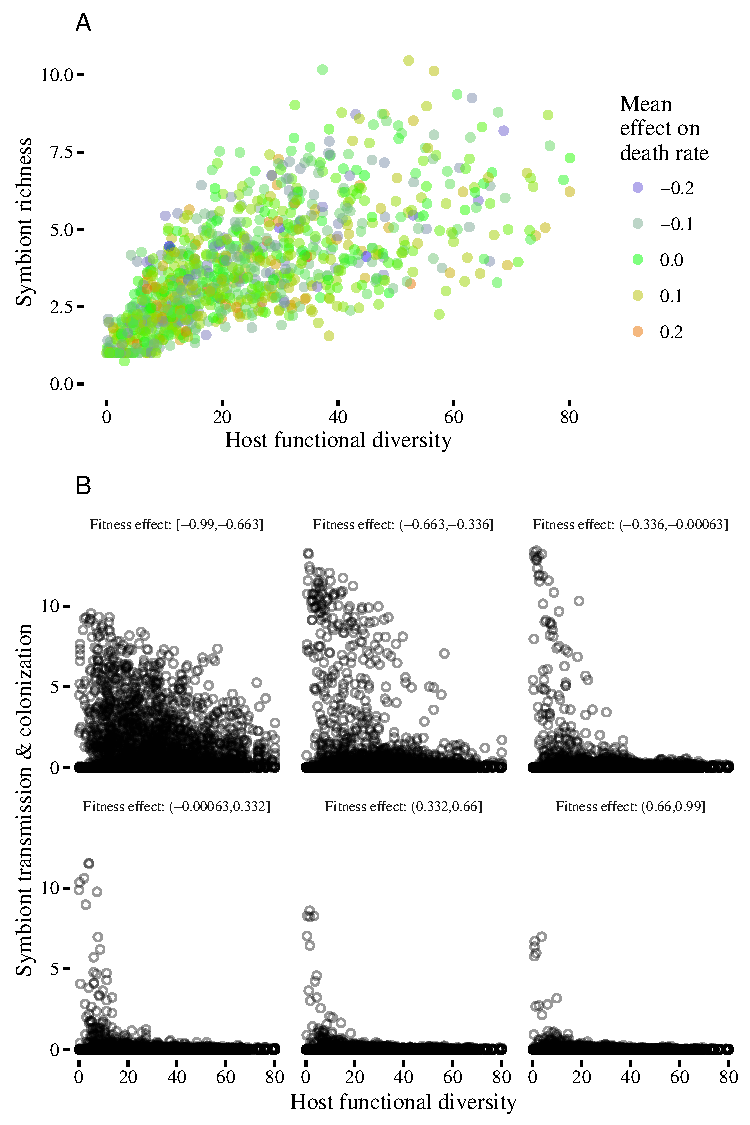
\includegraphics[width=\linewidth]{fig/fig5.pdf}
\caption{Mixed fitness consequences within symbiont community}
\label{fig:fig5}
\end{figure}

\newpage

\section*{Figure 6}

\begin{figure}[ht]\centering,
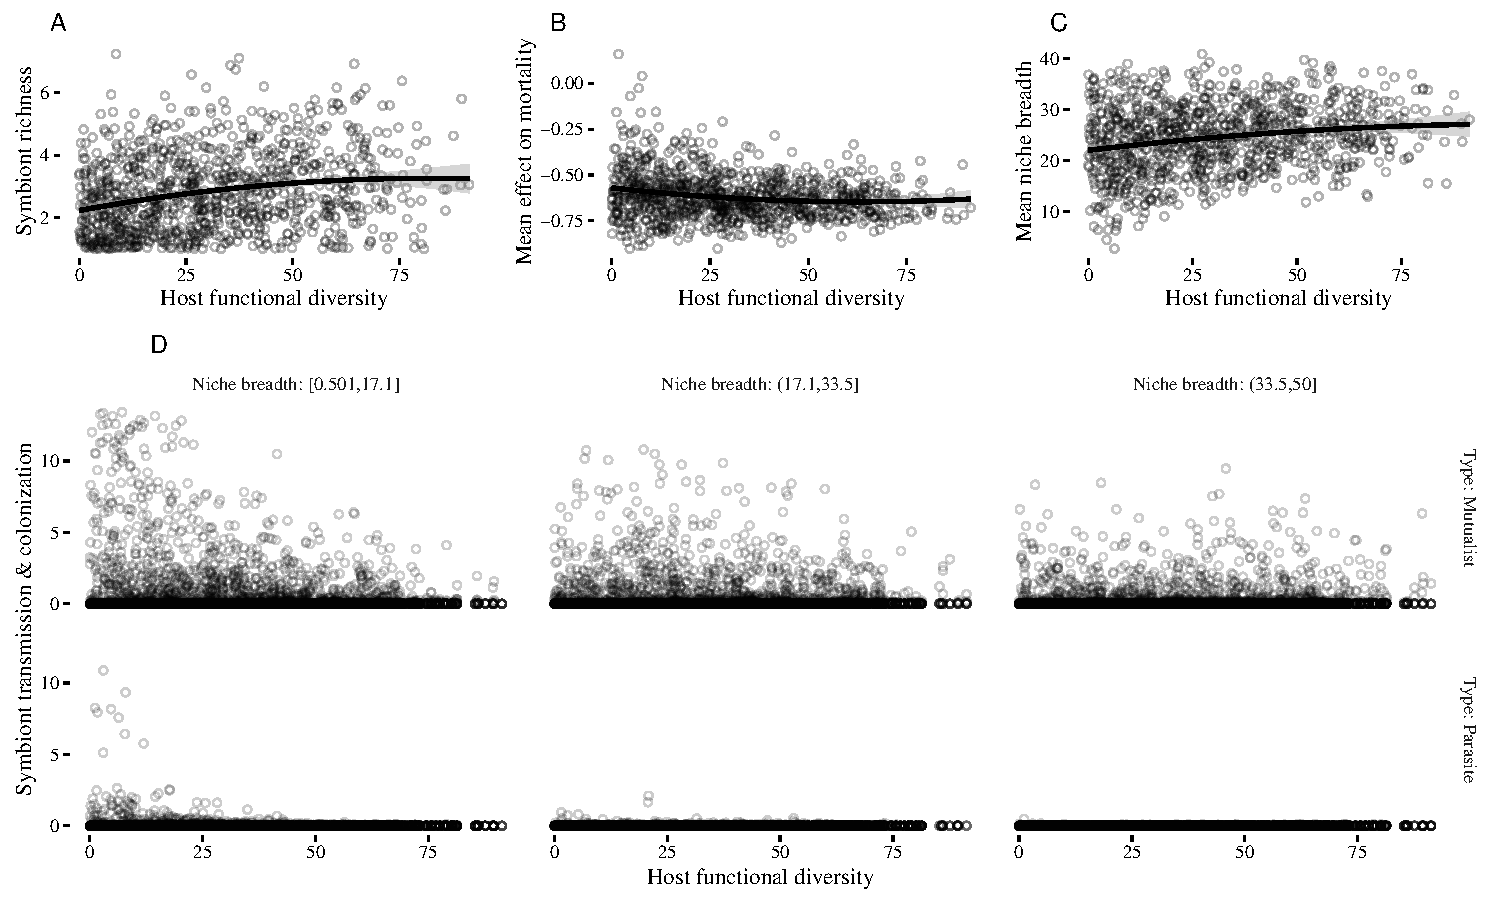
\includegraphics[width=\linewidth]{fig/fig6.pdf}
\caption{Mixed niche breadths and fitness consequences}
\label{fig:fig6}
\end{figure}

\end{document}